\chapter{Příprava dat}
V~této kapitole popíšeme, jak z~OSM dat vyrobíme graf pro vyhledávání pěších
tras. Nejprve z~dat vybereme pouze ta, která potřebujeme, a uložíme je do
našeho formátu k~dalšímu zpracování. Poté zjednodušíme budovy, rozdělíme příliš
dlouhé cesty, doplníme spojky mezi cestami, připravíme zkratky pro trasy přes
průchozí prostranství a nakonec ze všech dat vytvoříme vyhledávací graf.

\section{Klasifikace OSM dat} \label{label:kategorie}
V~našem formátu pro přípravu dat jsou cesty a multipolygony rozděleny do
kategorií podle toho, jaký druh skutečného objekt je jimi reprezentován. Cesty vzniklé
jako zkratky přes průchozí prostranství dostanou kategorii plochy, přes kterou
vedou. Když následně hledáme cestu, můžeme jednotlivým kategoriím přiřadit
rychlosti, jakými se po nich pohybujeme. Kategorie jsou následující:
\begin{itemize}
	\item \verb|WAY| -- cesta, o~které nic nevíme; rezervováno pro speciální
	případy
	\item \verb|WATER| -- strouha či přeskočitelný potok
	\item \verb|PARK| -- plocha s~udržovanou zelení, nízkou trávou
	\item \verb|GREEN| -- plocha s~neudržovanou zelení, často jsou v~ní
	prošlapané nezmapované cestičky
	\item \verb|FOREST| -- les v~městském slova smyslu, obvykle bývá pěšky
	průchozí
	\item \verb|PAVED| -- zpevněná cesta či plocha
	\item \verb|UNPAVED| -- nezpevněná cesta či plocha
	\item \verb|STEPS| -- schody
	\item \verb|HIGHWAY| -- silnice, silnice s~chodníkem
	\item \verb|BARRIER| -- překážka pro chodce nepřekonatelná, typ se
	nerozlišuje, například budova, řeka, plot, dálnice
	\item \verb|DIRECT| -- spojka mezi cestami -- krátké cesty generované
	pro doplnění chybějících napojení chodníků na silnice apod.
\end{itemize}
Rozdělení do kategorií probíhá s~pomocí konfiguračního souboru, ve kterém můžeme
zvolit jaké atributy mají objekty mít, aby patřily do dané kategorie. Protože
ani informace, zda jde o~plochu, není ve specifikaci OSM přesně definována, jsou
pro určení, zda jde o~plochu, použity údaje z~konfiguračního souboru. Po
rozdělení objektů do kategorií jsou smazány body, které neleží na žádné cestě,
protože takovéto body dále nikde nepotřebujeme.

\section{Převod multipolygonů na obvodové cesty}
Protože plochy popisované pomocí multipolygonů mají složitou strukturu a obtížně
by se nám s~nimi pracovalo, nahradíme multipolygony cestami reprezentujícími
vnější obvody jednotlivých komponent multipolygonů.

Abychom vytvořili obvody jednotlivých komponent, potřebujeme vědět, které cesty
patří do které komponenty.  Dokud nám nějaké cesty zbývají, skládáme z~nich
obvody komponent. Cesty na obvodu smažeme a nahradíme jednou uzavřenou cestou
reprezentující celý obvod komponenty. Pokud nemůžeme vytvořit ze zbývajících
cest kružnici -- obvod, pak vypíšeme chybu a multipolygon dále nezpracováváme.
Stejně se zachováme i v~případě, že kružnice končí v~jiném než počátečním bodě.
Obě tyto situace vznikají kvůli chybám ve zdrojových datech.

\section{Spojení budov}
Ve městě jsou velmi časté bloky budov. V~OSM datech jsou budovy obvykle reprezentovány
samostatně, přičemž nám stačí znát obvod celého bloku. Proto cesty
v~jednotlivých blocích nahradíme jednou cestou reprezentující obvod tohoto bloku.
Nejprve vybereme všechny budovy a vytvoříme si z~nich graf sousednosti
jednotlivých budov. Poté v~každé komponentě najdeme bod na obvodu a postupně
obejdeme po obvodu celou budovu a vytváříme při tom novou cestu. Původní
cesty budov potom smažeme. Když máme zpracované všechny budovy, smažeme body uvnitř
bloku, které nyní neleží na žádné cestě.

Při zpracování se mohou vyskytnout dva druhy problémů. Jednak se uvnitř bloků
mohou vyskytovat cesty, v~tom případě spojování cest přerušíme, protože bychom
se mohli připravit o~možnost přidání spojek mezi cestami uvnitř bloku. Druhý
problém souvisí s~problémem více bodů na stejných souřadnicích. V~případě, že
budovy nejsou zcela korektně navázané, vytvoříme z~nich korektní cestu, která
ale může obsahovat některé hrany navíc. Budovy také mohou mít na obvodu dva sousední body
na stejných souřadnicích. Pokud narazíme na tuto situaci, zjednodušování
ukončíme, protože nedokážeme určit, jestli tento bod leží na cestě tvořící
obvod, nebo na cestě vedoucí dovnitř budovy. Tento problém se ale nevyskytuje
příliš často, proto jsme ho speciálně neošetřovali.

\section{Rozdělení dlouhých úseků}
Pro další zpracování se nám bude hodit, abychom cesty, po kterých budeme
plánovat trasy, neměly příliš dlouhé úseky. Proto se na všechny takové cesty
podíváme a v~případě, že obsahují úseky delší než zvolená vzdálenost, tyto úseky
rovnoměrně rozdělíme na kratší. 

\section{Spojky mezi cestami}
Jak již bylo zmíněno, chodníky jsou v~OSM zmapovány jen některé a často nejsou
na sebe správně navázány. Proto jsme se rozhodli prohledat okolí každého uzlu a
spojit každé dva uzly, které jsou k~sobě blíže než 20\,m, úsečkou. Při zkoumání
OSM dat jsme zjistili, že mnohé obytné domy kolem sebe nemají značené ploty a
proto jsme vzdálenost zvolili takto nízkou, aby pravděpodobnost, že
jde například o~dvě ulice oddělené domky se zahrádkami, zůstala poměrně malá.  

V~oblastech, kde se nacházelo velké množstí uzlů blízko sebe, například u~cest
reprezentujících kruhové objezdy, vznikalo příliš velké množství spojek. Tyto
spojky navíc nepřinášely významné zkrácení trasy. U~každého uzlu jsme proto
náhodně vybrali jen některé spojky (viz obr. \ref{fig:spojky}.

\begin{figure}[h]
	\centering
	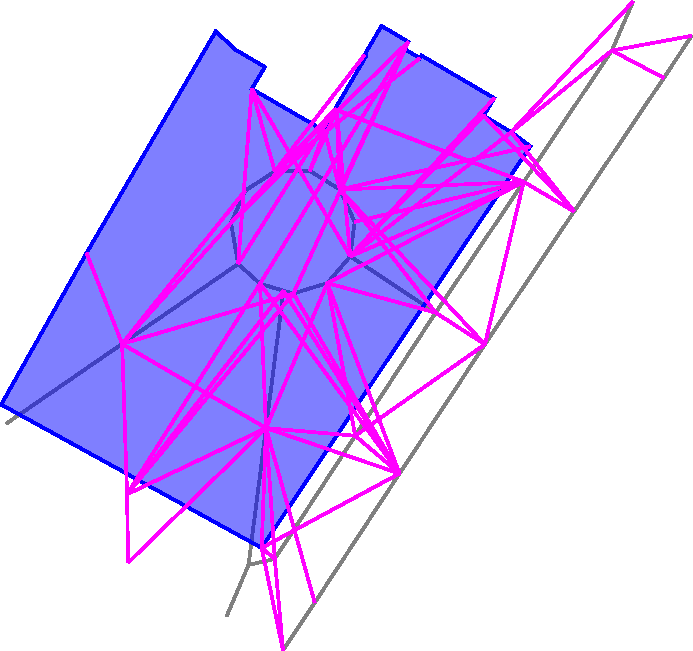
\includegraphics{../img/spojky.pdf}
	\caption{Spojky na malém území. Pokud bychom zde nevybírali náhodně, získali
	bychom velké množství spojek, které by zkrácení trasy příliš nepomohly.
	Růžové úsečky značí vytvořené spojky po náhodném výběru.}
	\label{fig:spojky}
\end{figure}

Spojky navíc mohou vést přes nějakou překážku, jako je plot nebo zeď, proto
potřebujeme zkontrolovat kolize všech přidaných spojek s~překážkami. K~tomuto
účelu jsme využili algoritmus využívající zametání roviny.


{\tuc Zametání roviny} \cite{zametani} je způsob návrhu geometrického algoritmu,
při němž rovinou posouváme přímku (\uv{zametáme}). Pokud přímka protne pro nás
zajímavé místo, vyvoláme událost. Během procházení si obvykle navíc pamatujeme
seznam prošlých bodů nebo aktuálně protnutých úseček, tzv. {\tuc průřez}.

V~našem případě budeme hledat průsečíky úseček v~rovině. Spojky již úsečky jsou,
překážky rozdělíme na jednotlivé úsečky mezi uzly. Budeme zametat podle od
západu k~východu a zajímat nás budou události začátku a konce úsečky a jejich
průsečík. Zametací přímku proto budeme posouvat postupně po těchto událostech.

Začátky a konce úseček známe již před spuštěním algoritmu. Průsečíky na začátku
neznáme, budeme ale předpokládat, že se neprotínají tři úsečky v~jednom bodě.
Potom platí, že pokud se nějaké dvě úsečky mají protnout, pak se předtím musí
stát sousedními. Proto nám stačí při každé události s~úsečkou $u$ stačí
zkontrolovat sousedy $u$ a pokud se s~nějakým protíná a průsečík je před
zametací přímkou, přidáme ho do seznamu událostí.

\begin{figure}[h]
	\centering
	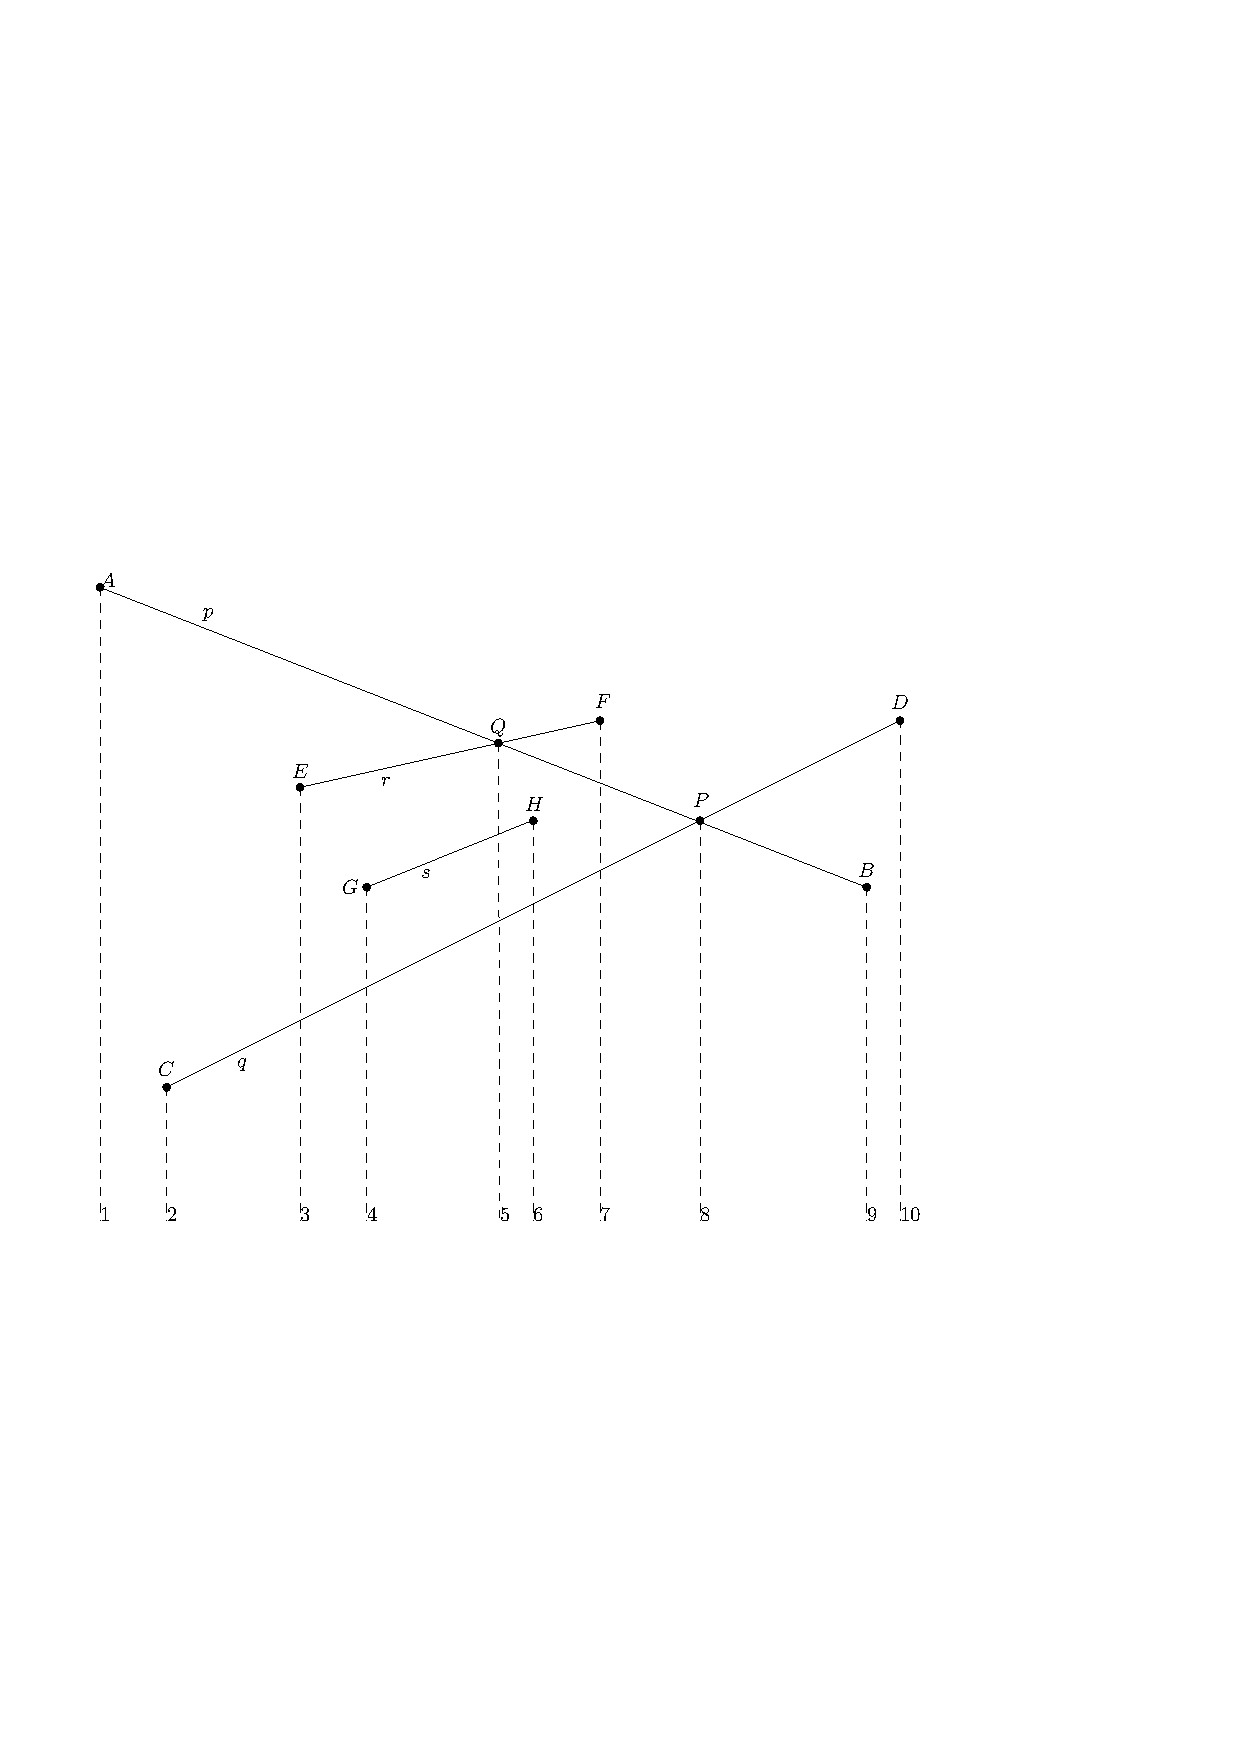
\includegraphics{../img/zametani.pdf}
	\caption{Zametání roviny}
	\label{fig:zametani}
\end{figure}

Protože vždy budeme potřebovat znát nejbližší událost, budeme si udržovat
události v~haldě. Dále také potřebujeme znát pořadí, v~jakém aktuálně
zpracovávané úsečky protínají rovinu -- průřez, a umět mezi ně přidat další a
odebrat tu, která skončí. K~tomuto účelu se nám hodí použít vyhledávací strom.
Nemůžeme si ovšem ve vrcholech pamatovat přímo souřadnice průsečíku úsečky se
zametací přímkou, protože se tyto souřadnice mění s~každým posunutím zametací
přímky. Místo toho si budeme ve stromě pamatovat jen odkazy na úsečky a průsečíky
budeme počítat, až to bude potřeba.

Na začátku známe všechny začátky a konce úseček, vytvoříme tedy v~haldě události
začátků a konců úseček. Průsečíkové události zatím žádné neznáme, ale protože
aby mohl nastat průsečík, musí nejprve úsečka začít, o~žádný nepřijdeme.

Zametání ukázkových dat se čtyřmi úsečkami ukazuje obrázek \ref{fig:zametani}.
Svislé přerušované čáry udávají pozice zametací přímky při vyvolání události,
události nastávají v~pořadí 1 až 10.

Zametání bude probíhat následovně. Z~haldy všech událostí vybereme nejbližší
událost a rozhodneme se podle jejího typu:
\begin{itemize}
	\item {\tuc Začátek úsečky.}  Úsečku zařadíme na správné místo do
	průřezu a přidáme případné průsečíkové události se sousedními
	úsečkami.\\
	V~situacích 1 a 4 úsečku pouze přidáme, k~průsečíkům nedochází.\\
	V~situacích 2 a 3 se úsečky protínají, přidáme průsečíkové události
	$P$ a $Q$.

	\item {\tuc Konec úsečky.} Úsečku odebereme z~průřezu a přidáme
	případnou průsečíkovou událost, pokud se úsečky sousední s~právě
	končící protínají.\\
	V~situacích 7, 9 a 10 pouze úsečky odebereme z~průřezu.\\
	V~situaci 6 se po skončení úsečky $s$ stanou úsečky $p$ a $q$ sousedními
	a navíc se protínají, proto přidáme průsečíkovou událost $P$.
	\item {\tuc Průsečík úseček.} Úsečky v~průřezu prohodíme a přidáme
	případné průsečíkové události s~novými sousedy obou prohazovaných 
	úseček. Pokud jsme již průsečík těchto dvou úseček zpracovávali, událost
	zahodíme, protože úsečky se mohou protnout nejvýše jednou a další události
	jsou pouze násobným přidáním téže události (jako zde průsečíku $P$).\\
	V~situaci 8 nemají prohozené úsečky žádné nové sousedy.\\
	V~situaci 5 se nově stala úsečka $s$ sousedem prohozené přímky $p$, ale
	nemají společný průsečík, událost tedy nepřidáváme.
\end{itemize}
Takto budeme postupovat, dokud jsou v~haldě nějaké události. Pokud zpracováváme 
průsečíkovou událost, zkontrolujeme, zda není některá z~úseček překážka a 
případně úsečky označíme, že se protnuly s~překážkou. 


\section{Zkratky přes průchozí prostranství}
Pokud procházíme ve městě přes větší park nebo náměstí, často nemusíme chodit
jen po chodnících, ale můžeme projít přes prostranství přímo. Přímé cesty přes
průchozí prostranství proto také chceme zanést do vyhledávacího grafu. K~jejich
vytvoření jsme využili modifikovaný algoritmus vytváření spojek mezi cestami.
Dvojice bodů v~průchozích prostranstvích jsme spojovali úsečkami. Tentokrát jsme
ale hledali dvojice bližší než 300 m, protože parky mohou být poměrně rozlehlé.
Opět jsme nepoužívali všechny dvojice ale jen některé náhodně vybrané, protože
jinak vznikalo příliš mnoho úseček, které vedly podobně, a proto nepřinášely
významné zlepšení vyhledané trasy. Protože i na průchozích prostranstvích se
vyskytují překážky, opět jsme pomocí zametání roviny odstranili všechny úsečky,
které procházely přes nějakou překážku.

\section{Vytvoření vyhledávacího grafu}
Poté, co jsme připravili data, vytvoříme vyhledávací graf. Protože kolize
přímých cest s~překážkami jsme vyřešili již při jejich vytváření, jsou všechny
cesty korektní. Proto se překážkami již dále nezabýváme a pouze z~cest vytvoříme
vyhledávací graf. Pokud byly v~datech přítomny cesty nepřipojené ke zbytku a ani 
přidání spojek a zkratek je nepřipojilo, měl by tento graf více komponent. Tyto
převážně malé komponenty nás nezajímají, protože do nich neumíme najít cestu, a
proto použijeme jen největší komponentu. Uložíme seznam všech uzlů, které jsou
na jejích cestách použity a cesty rozdělíme na jednotlivé hrany grafu mezi dvěma
uzly.  U~hran zachováme údaje o~typu cesty, protože je budeme využívat při
vyhledávání.
